\documentclass[12pt]{article}
\usepackage[margin=1in]{geometry}
\usepackage{graphicx}
\usepackage{amsmath}
\usepackage{booktabs}
\usepackage{float}
\usepackage{xcolor}

% placeholders for text still to be written - delete the \todo once filled in
\newcommand{\todo}[1]{\textcolor{red}{\textbf{[WRITE HERE:} \textit{#1}\textbf{]}}}

\title{}
\date{}

\begin{document}

% ---------- Title page ----------
\begin{titlepage}
\centering
\vspace*{2cm}
{\Large \textbf{ASSIGNMENT REPORT-2}}\\[2cm]

\textbf{Submitted by :}\\[0.3cm]
\textbf{KARTHIKEYAN M} \ [26120004]\\[0.3cm]
\textbf{MIRTHULA R} \ [261200121]\\[2cm]

\textbf{Under the guidance of :}\\[0.3cm]
\textbf{HEMA ARUNACHALAM MURTHY}\\[1.5cm]

\textbf{For The Subject}\\[0.5cm]
{\Large \textbf{Pattern Recognition and Machine Learning}}\\[0.3cm]
\textbf{(26AI5707)}\\[3cm]

\vfill

\textbf{DEPARTMENT OF COMPUTER SCIENCE \& ENGINEERING}\\[0.3cm]
\textbf{SHIV NADAR UNIVERSITY}\\[0.3cm]
\textbf{KALAVAKAM}\\[1.5cm]

\textbf{AUGUST 2026}

\end{titlepage}

% ---------- Introduction ----------
\section*{INTRODUCTION:}

This lab is all about dimensionality reduction. We use decomposition techniques
such as eigenvalue decomposition (diagonalization) and singular value
decomposition to decompose an image and try to reconstruct it with fewer
dimensions than the original amount. The square image gets both EVD and SVD,
while the rectangular image only gets SVD. Both these techniques do the similar thing: they decompose the matrix (image
representation) into its eigenvalues/eigenvectors or singular values/vectors,
and then try to reconstruct the original image with as few of these as
possible. This makes a compressed, approximate form of the image.

% ---------- Experiments Performed ----------
\section*{Experiments Performed:}

\subsection*{Question 1: Square image (EVD + SVD)}

\textbf{Pipeline.}
\begin{itemize}
  \item \textbf{Load:} first we use matplotlib image to load the image.
  \item \textbf{Resize:} then we resize it to $100\times100$ (it's a square
        image, so both sides just become 100).
  \item \textbf{Grayscale:} we convert it into grayscale by extracting the
        RGB channels and using the arithmetic formula
        $0.299R + 0.587G + 0.114B$.
\end{itemize}
Then we perform the decomposition and reconstruct using different values of $k$.

\begin{figure}[H]
\centering
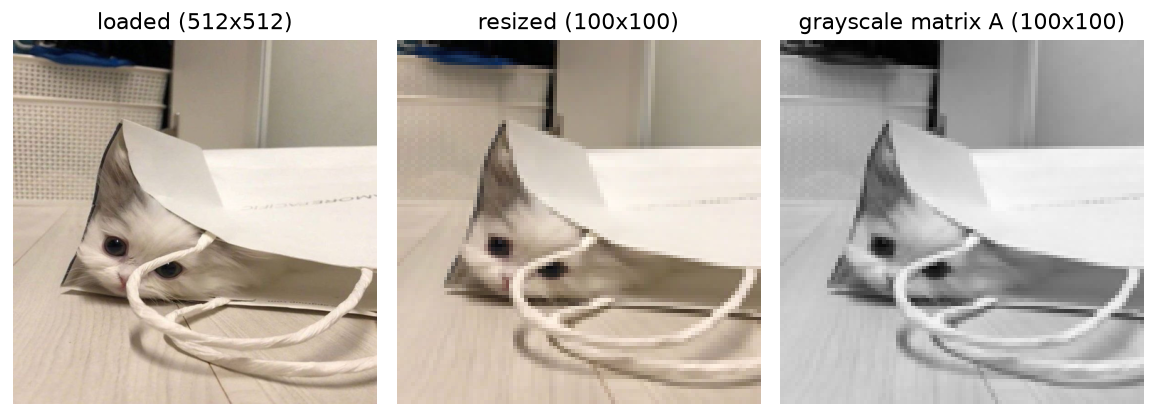
\includegraphics[width=0.9\textwidth]{figures/square_pipeline.png}
\caption{Load $\rightarrow$ resize $\rightarrow$ grayscale, square image ($A$ is $100\times100$, values in $[0,255]$).}
\end{figure}

\textbf{EVD.} Eigenvalue decomposition, also known as diagonalization, is a
process used to decompose a square matrix into a diagonal matrix $\Lambda$
and its eigenbasis:
\begin{equation}
A = Q\Lambda Q^{-1}
\end{equation}
Here $Q$ contains the eigenbasis (the eigenvectors) and $\Lambda$ is the
diagonal matrix containing the eigenvalues. There are multiple reasons we do
this, one of them being to study the matrix through its eigenvalues and
eigenvectors.

\textbf{SVD.} While diagonalization is helpful, it can only be performed on
square matrices. SVD extends this idea to non-square matrices:
\begin{equation}
A = U\Sigma V^t
\end{equation}
We have two matrices, $AA^T$ giving us eigenvalues and corresponding
eigenvectors stacked in $U$, and $A^TA$ giving us eigenvalues and
corresponding eigenvectors stacked in $V$. $\Sigma$ is the singular value
matrix, sharing the same dimensions as $A$, containing the singular values,
and singular values are the square root of the eigenvalues. The basic idea
is that a non-square matrix cannot be diagonalized directly, so $AA^T$ and
$A^TA$ are used to make it square first.

\textbf{Choice of $k$.} We chose $k = 5, 20, 50$: jumping from a very low
point ($k=5$, heavy compression) up to $k=50$ (half the image's dimension),
with $k=20$ in between, to show the difference in errors across that range.

\begin{figure}[H]
\centering

\includegraphics[width=0.75\textwidth]{figures/square_evd_5.png}\\
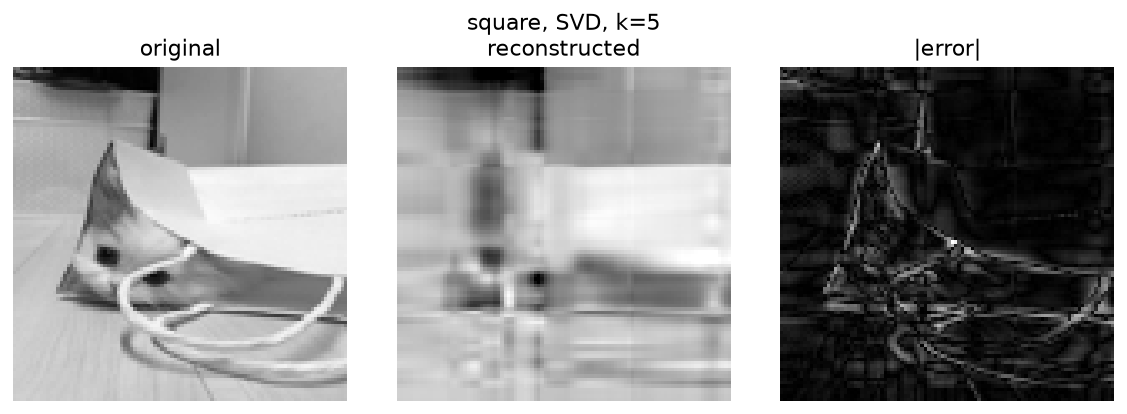
\includegraphics[width=0.75\textwidth]{figures/square_svd_5.png}
\caption{Square image, $k=5$: EVD (top) vs SVD (bottom).}
\end{figure}

\begin{figure}[H]
\centering
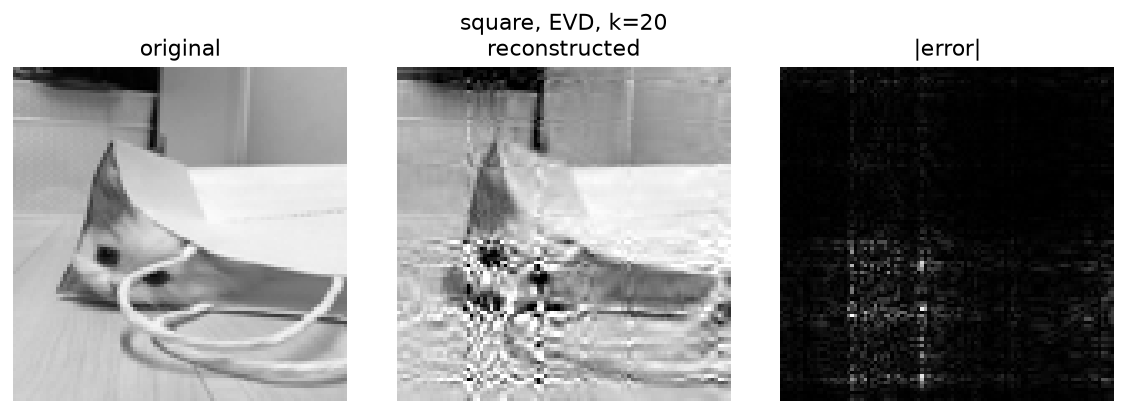
\includegraphics[width=0.75\textwidth]{figures/square_evd_20.png}\\
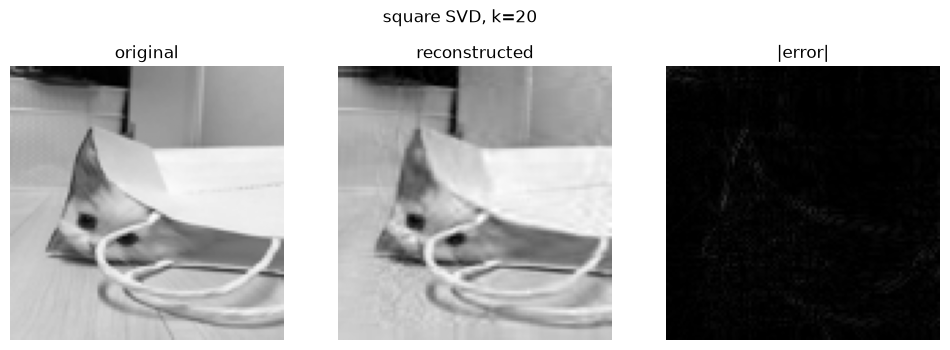
\includegraphics[width=0.75\textwidth]{figures/square_svd_20.png}
\caption{Square image, $k=20$: EVD (top) vs SVD (bottom).}
\end{figure}

\begin{figure}[H]
\centering
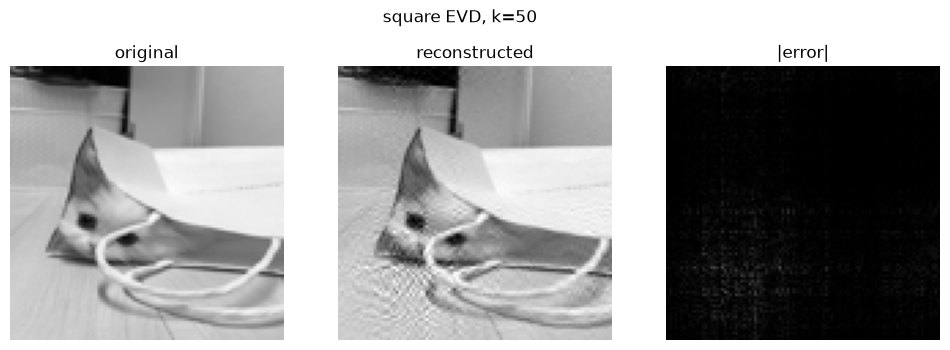
\includegraphics[width=0.75\textwidth]{figures/square_evd_50.png}\\
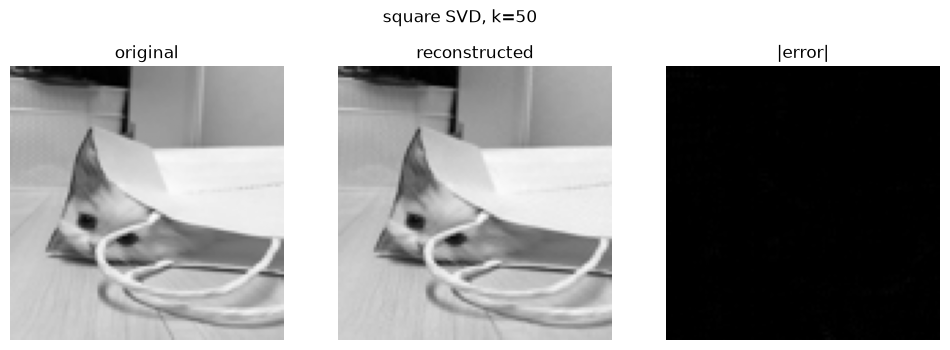
\includegraphics[width=0.75\textwidth]{figures/square_svd_50.png}
\caption{Square image, $k=50$: EVD (top) vs SVD (bottom).}
\end{figure}

SVD performs considerably better than EVD, even for this square image. SVD's
$U$ and $V$ are orthogonal no matter what $A$ looks like. $Q$, on the other
hand, is only orthogonal when $A$ itself is symmetric, but it's not in our
case, so orthogonality is causing the difference there.

\begin{table}[H]
\centering
\begin{tabular}{cccc}
\toprule
$k$ & $E(k)$ EVD & $E(k)$ SVD & ratio \\
\midrule
5  & 3281.02 & 1736.93 & $\sim$1.9x \\
20 & 2575.44 & 581.84  & $\sim$4.4x \\
50 & 765.98  & 122.67  & $\sim$6.2x \\
\bottomrule
\end{tabular}
\caption{Reconstruction error, square image.}
\end{table}

SVD's error is consistently lower than EVD's at every $k$, and the gap
actually widens as $k$ grows ($\sim$1.9x at $k=5$ up to $\sim$6.2x at
$k=50$).

\begin{figure}[H]
\centering
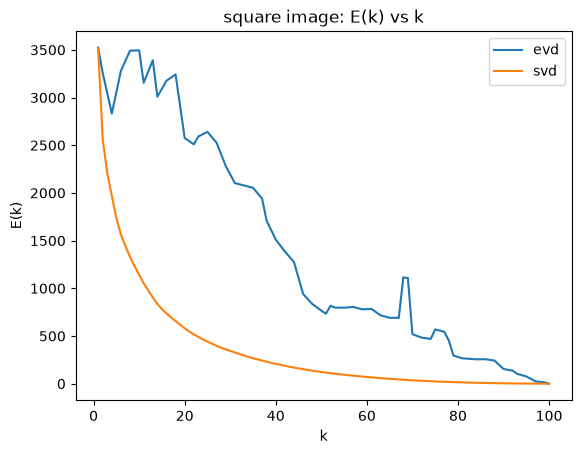
\includegraphics[width=0.7\textwidth]{figures/square_curve.png}
\caption{$E(k)$ vs $k$, square image, all $k$ from 1 to 100.}
\end{figure}

SVD guarantees orthogonality. The orthogonal vectors are perpendicular to
each other, so none of them overlap, and each one is new information on its
own. When you keep the important ones and drop the smaller, unwanted ones,
the error visibly drops. That is why EVD's error fluctuates a little instead
of gradually decreasing, while SVD's error gradually decreases.

\textbf{Complex eigenvalues.} 82 out of 100 eigenvalues came out complex.
This is because $A$ isn't symmetric, so the characteristic polynomial's
roots aren't guaranteed to be real, and it splits out complex numbers
instead. In the code, this is handled by not splitting conjugate pairs
across the $k$ boundary when truncating, and then stripping out the
imaginary part and keeping only the real part before the result becomes a
displayable image.

\subsection*{A Deep look into EVD at $k=20$}

\[
A \;=\; \sum_{i=1}^{100} \lambda_i \, q_i r_i ,
\qquad
\text{layer size} \;=\; \lVert \lambda_i q_i r_i \rVert_F \;=\; |\lambda_i| \cdot \lVert q_i \rVert \cdot \lVert r_i \rVert
\]

where, for each $i$,
\begin{itemize}
\itemsep0em
\item $\lambda_i$ is the $i$-th eigenvalue of $A$,
\item $q_i$ is the $i$-th column of $Q$, i.e. the eigenvector for $\lambda_i$,
\item $r_i$ is the $i$-th row of $Q^{-1}$,
\item $\mathrm{gap}_i = \min_{j \neq i} |\lambda_i - \lambda_j|$ is the straight-line
      distance in the complex plane from $\lambda_i$ to the nearest other eigenvalue.
      For a conjugate pair $a \pm bi$ the two members are $2|b|$ apart, so the gap is
      set by the size of the imaginary part.
\end{itemize}

\begin{table}[H]
\centering
\small
\setlength{\tabcolsep}{4pt}
\begin{tabular}{clccccc}
\toprule
$i$ & \multicolumn{1}{c}{$\lambda_i$} & $|\lambda_i|$ & $\lVert q_i \rVert$ & $\lVert r_i \rVert$ & $\mathrm{gap}_i$ & layer size \\
\midrule
0  & 17299.45          & 17299.5 & 1.0 & 1.0  & 16990.1 & 17685 \\
1  & -976.95           & 977.0   & 1.0 & 3.4  & 538.3   & 3293  \\
2  & -476.72 + 198.85i & 516.5   & 1.0 & 4.1  & 336.0   & 2138  \\
3  & -476.72 - 198.85i & 516.5   & 1.0 & 4.1  & 336.0   & 2138  \\
4  & 241.92 + 316.27i  & 398.2   & 1.0 & 4.7  & 238.9   & 1886  \\
5  & 241.92 - 316.27i  & 398.2   & 1.0 & 4.7  & 238.9   & 1886  \\
6  & 309.62 + 87.19i   & 321.7   & 1.0 & 10.0 & 154.2   & 3212  \\
7  & 309.62 - 87.19i   & 321.7   & 1.0 & 10.0 & 154.2   & 3212  \\
8  & -66.15 + 225.62i  & 235.1   & 1.0 & 5.3  & 135.1   & 1256  \\
9  & -66.15 - 225.62i  & 235.1   & 1.0 & 5.3  & 135.1   & 1256  \\
10 & 182.44            & 182.4   & 1.0 & 10.1 & 66.6    & 1851  \\
11 & -171.43 - 58.55i  & 181.2   & 1.0 & 10.3 & 58.8    & 1858  \\
12 & -171.43 + 58.55i  & 181.2   & 1.0 & 10.3 & 58.8    & 1858  \\
13 & -177.14           & 177.1   & 1.0 & 8.5  & 58.8    & 1503  \\
14 & 97.03 + 89.13i    & 131.8   & 1.0 & 10.2 & 60.8    & 1348  \\
15 & 97.03 - 89.13i    & 131.8   & 1.0 & 10.2 & 60.8    & 1348  \\
16 & 32.23 + 117.24i   & 121.6   & 1.0 & 12.4 & 28.5    & 1513  \\
17 & 32.23 - 117.24i   & 121.6   & 1.0 & 12.4 & 28.5    & 1513  \\
\textbf{18} & \textbf{115.92 + 3.91i} & \textbf{116.0} & \textbf{1.0} & \textbf{88.8} & \textbf{7.8} & \textbf{10297} \\
\textbf{19} & \textbf{115.92 - 3.91i} & \textbf{116.0} & \textbf{1.0} & \textbf{88.8} & \textbf{7.8} & \textbf{10297} \\
\midrule
20 & -26.14 + 96.61i   & 100.1   & 1.0 & 10.3 & 26.2    & 1027  \\
21 & -26.14 - 96.61i   & 100.1   & 1.0 & 10.3 & 26.2    & 1027  \\
\bottomrule
\end{tabular}
\caption{The 20 EVD layers kept at $k=20$}
\end{table}

Each term in the summation is just an outer-product between columns of $Q$ and rows of $Q^{-1}$ and scaled by the corresponding eigen value. If you look at the eigen values at the $18^{th}$ and $19^{th}$ you could see they are very close to each other as the imaginary part is very low and they have huge layer size. (i.e.) 10297 the second largest after our largest eigen value's layer size. So, we are essentially not preserving the balance effect after truncating to just k values.

\subsection*{Question 2: Rectangular image (SVD only)}

EVD can only handle square matrices and can't handle non-square matrices.
That's the main reason why we have SVD in the first place.

From the image, the width and height are extracted, and then the maximum
side is fixed to 100 and the other side is resized to maintain the aspect
ratio using (min\_side $\times$ 100 / max\_side).

\begin{figure}[H]
\centering
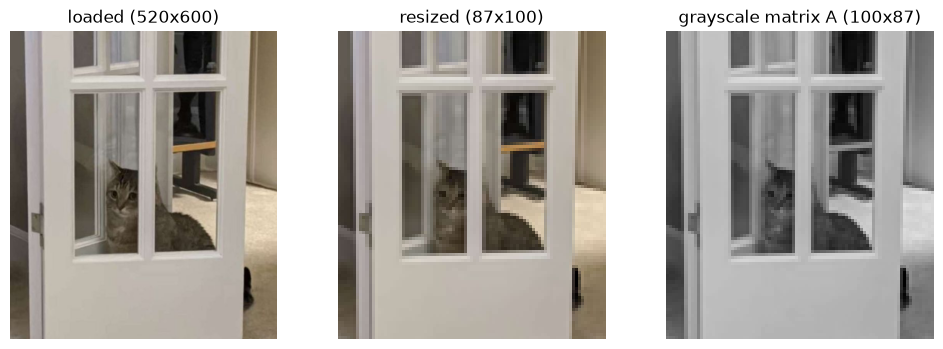
\includegraphics[width=0.9\textwidth]{figures/rect_pipeline.png}
\caption{Load $\rightarrow$ resize (aspect-preserving) $\rightarrow$ grayscale, rectangular image ($520\times600 \rightarrow 87\times100$).}
\end{figure}

\begin{figure}[H]
\centering
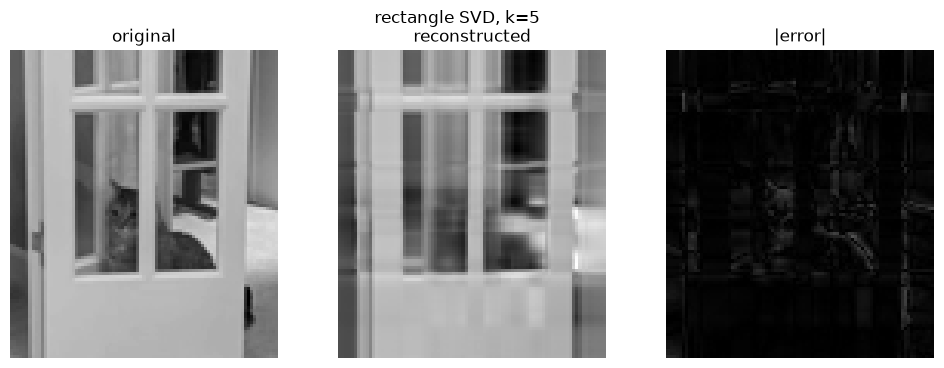
\includegraphics[width=0.75\textwidth]{figures/rect_svd_5.png}
\caption{Rectangular image, SVD, $k=5$.}
\end{figure}

\begin{figure}[H]
\centering

\includegraphics[width=0.75\textwidth]{figures/rect_svd_20.png}
\caption{Rectangular image, SVD, $k=20$.}
\end{figure}

\begin{figure}[H]
\centering

\includegraphics[width=0.75\textwidth]{figures/rect_svd_50.png}
\caption{Rectangular image, SVD, $k=50$.}
\end{figure}

\begin{table}[H]
\centering
\begin{tabular}{cc}
\toprule
$k$ & $E(k)$ SVD \\
\midrule
5  & 1100.14 \\
20 & 251.75 \\
50 & 34.15 \\
\bottomrule
\end{tabular}
\caption{Reconstruction error, rectangular image.}
\end{table}

The error drops gradually and smoothly as $k$ increases, the same monotonic
behaviour SVD showed on the square image.

\begin{figure}[H]
\centering
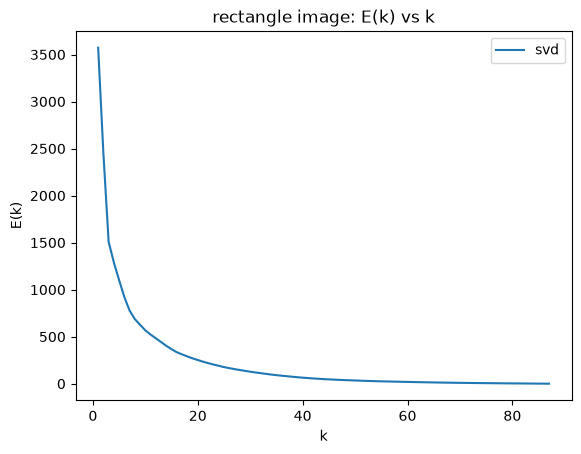
\includegraphics[width=0.7\textwidth]{figures/rect_curve.png}
\caption{$E(k)$ vs $k$, rectangular image, all $k$ from 1 to 87.}
\end{figure}

% ---------- Inference ----------
\section*{\centering \underline{Inference}}

If it's a square matrix and symmetric already, just go with EVD because it's
less computationally complex than SVD. Reach for SVD whenever there is a
need to handle non-square matrices.

Complex eigenvalues really took its time to land. We pondered a lot just to
end up getting the justification from the quadratic roots formula.

\end{document}